\vspace*{1em}

Fix sets $A,\,B$. For a visual motivation, we view the cartesian product $A \times B$ as a plane with the horizontal axis represented by $A$ and the vertical axis represented by $B$. 
\[\begin{tikzpicture}
	\draw[<->,thick] (-0.5,0) -- (2.5,0) node[right] {$A$};
	\draw[<->,thick] (0,-0.5) -- (0,2.5) node[above] {$B$};
\end{tikzpicture}\]
This in no way rigorously reflects the set $A \times B$ but is useful in getting a sense of definitions and notions we will see.

\vspace*{1em}

\begin{definition}
A \cdef{relation} from $A$ to $B$ is a subset of $A \times B$.\\
\\
For a relation $R \subseteq A \times B$, given any element $(a,b) \in R$, we write $aRb$ and say \[\text{\emph{$a$ is $R$-related to $b$}}\]
If $(a,b) \notin R$, then we write $a \cancel{R} b$ and say \emph{$a$ is not $R$-related to $b$}.
\end{definition}

\vspace*{1em}

\begin{example}\hfill
\begin{itemize}[itemsep=1em]
\item[(1)] Let $f: A \times B$ be a function, let $\Gamma(f)$ be its graph
\[\Gamma(f) = \setp{(a,f(a))}{a \in A} \subseteq A \times B\]
\[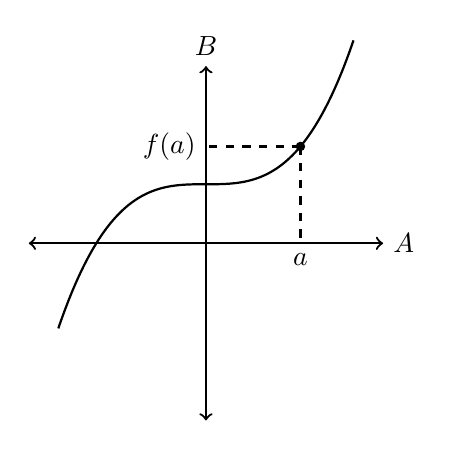
\begin{tikzpicture}[scale=1.5]
	\draw[<->,thick] (-1.5,0) -- (1.5,0) node[right] {$A$};
	\draw[<->,thick] (0,-1.5) -- (0,1.5) node[above] {$B$};
	\draw[thick, domain=-1.25:1.25, samples=200, variable=\x] plot (\x, {(5*\x^3 + 4)/8});
	\filldraw (0.8,0.82) circle (1pt);
	\draw[thick,dashed] (0.8,0.82) -- (0,0.82) node[left] {$f(a)$};
	\draw[thick,dashed] (0.8,0.82) -- (0.8,0) node[below] {$a$};
\end{tikzpicture}\]
This is a relation from $A$ to $B$. In this way, a function is a special case of a relation.

\item[(2)] Let 
\[S = \setp{(x,y) \in \rr^2}{x^2 + y^2 = 1} \subseteq \rr \times \rr,\]
this is a relation from $\rr$ to $\rr$.
\[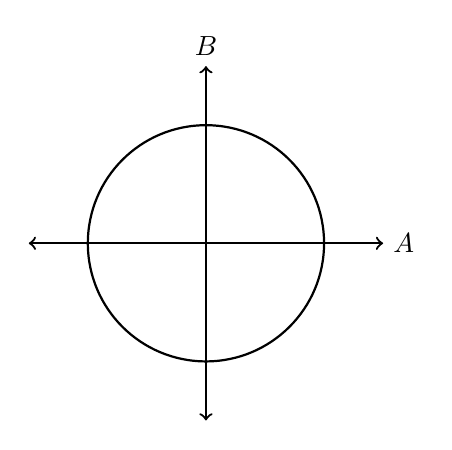
\begin{tikzpicture}[scale=1.5]
	\draw[<->,thick] (-1.5,0) -- (1.5,0) node[right] {$A$};
	\draw[<->,thick] (0,-1.5) -- (0,1.5) node[above] {$B$};
	\draw[thick] (0,0) circle (1);
\end{tikzpicture}\]
Solving for $y$ gives \[y = \pm \sqrt{1 - x^2}\]
This is a \emph{multi-valued function} (fails the vertical line test) defined on $[-1,1]$. We usually do not call such things functions, but it is a legitimate relation on $\rr$.
\end{itemize}
\end{example}

\vspace*{1em}

\begin{definition}
Let $R \subseteq A \times B$ be a relation from $A$ to $B$. The \cdef{domain\ of} {\color{blue}$R$} is
\[\dom(R) = \setp{a \in A}{(a,b) \in R \text{ for some $b \in B$}}\]
This is the set of all first coordinates that occur in elements of $R$.\\
\\
The \cdef{range\ of} {\color{blue}$R$} (also called \cdef{image\ of} {\color{blue}$R$}) is
\[\range(R) = \setp{b \in B}{(a,b) \in R \text{ for some $a \in A$}}\]
This is the set of all second coordinates that occur in elements of $R$.\\
\\
Visually, for example,
\[\begin{tikzpicture}[scale=1.1]
    \draw[<->,thick] (-1,0)--(4.5,0) node[right] {$A$};
	\draw[<->,thick] (0,-1)--(0,4.5) node[above] {$B$};
    \node[] at (3.15,3) {$R$};
    
    \path[draw,thick,use Hobby shortcut,closed=true,fill=forest,fill opacity=1/10]
(1,1) .. (2,0.5) .. (3,1) .. (4,3) .. (3,4) .. (2,2) .. (1,1);

	\draw[thick,dashed,newblue] (0.985,2) -- (0.985,0);
	\draw[thick,dashed,newblue] (4.015,4.5) -- (4.015,0);
	\draw[thick,dashed,firebrick] (4.5,4.025) -- (0,4.025);
	\draw[thick,dashed,firebrick] (3,0.475) -- (0,0.45);
	
	\draw [decorate,decoration={brace,amplitude=10pt,mirror,raise=4pt},yshift=0pt,thick,newblue]
(0.985,0) -- (4.015,0) node [black,midway,below,yshift=-1.5em] {\small$\color{newblue}\dom(R)$};
	\draw [decorate,decoration={brace,amplitude=10pt,mirror,raise=4pt},yshift=0pt,thick,firebrick]
(0,4.025) -- (0,0.45) node [black,midway,left,xshift=-1.5em] {\small$\color{firebrick}\range(R)$};

    \node[right] at (4.15,2.25) {$\Downarrow$ project onto $A$};
    \node[above] at (2,4.2) {$\Leftarrow$ project onto $B$};

\end{tikzpicture}\]
\end{definition}

%\vspace*{1em}

\begin{definition}
Let $R \subseteq A \times B$ be a relation from $A$ to $B$. The \cdef{inverse\ relation} {\color{blue}$R^{-1}$} is
\[R^{-1} = \setp{(b,a) \in B \times A}{(a,b) \in R},\]
a relation from $B$ to $A$.
Visually, for example,
\[\begin{tikzpicture}
    \draw[<->,thick] (-1,0)--(4.5,0) node[right] {$A$};
	\draw[<->,thick] (0,-1)--(0,4.5) node[above] {$B$};
    \node[above] at (3.2,4) {$R$};
    
    \path[draw,thick,use Hobby shortcut,closed=true,fill=forest,fill opacity=1/10]
(1,1) .. (2,0.5) .. (3,1) .. (4,3) .. (3,4) .. (2,2) .. (1,1);

	\filldraw (3.25,2) circle (1.5pt) node[above] {\small$(a,b)$};
	\draw[thick,dashed] (3.25,2) -- (3.25,0) node[below] {\small $a$};
	\draw[thick,dashed] (3.25,2) -- (0,2) node[left] {\small $b$};
	\filldraw (3.25,0) circle (1.5pt);
	\filldraw (0,2) circle (1.5pt);
\end{tikzpicture}
\qquad
\begin{tikzpicture}
    \draw[<->,thick] (-1,0)--(4.5,0) node[right] {$B$};
	\draw[<->,thick] (0,-1)--(0,4.5) node[above] {$A$};
    \node[right] at (4,3.2) {$R^{-1}$};
    
    \path[draw,thick,use Hobby shortcut,closed=true,fill=forest,fill opacity=1/10]
(1,1) .. (0.5,2) .. (1,3) .. (3,4) .. (4,3) .. (2,2) .. (1,1);

	\filldraw (2,3.25) circle (1.5pt) node[right] {\small$(b,a)$};
	\draw[thick,dashed] (2,3.25) -- (0,3.25) node[left] {\small $a$};
	\draw[thick,dashed] (2,3.25) -- (2,0) node[below] {\small $b$};
	\filldraw (0,3.25) circle (1.5pt);
	\filldraw (2,0) circle (1.5pt);
\end{tikzpicture}
\]
If $A = B$, then we obtain $R^{-1}$ by reflecting along the \emph{diagonal}, this is the subset defined as \[\Delta_A = \setp{(a,a)}{a \in A} \subseteq A \times A.\]
\[\begin{tikzpicture}
    \draw[<->,thick] (-1,0)--(4.5,0) node[right] {$A$};
	\draw[<->,thick] (0,-1)--(0,4.5) node[above] {$A$};
	\draw[<->,thick] (-0.5,-0.5)--(4.5,4.5) node[above right] {$\Delta_A$};
    \node[right] at (4.5,1.5) {$R$};
    \node[above] at (1.5,4.5) {$R^{-1}$};
    
    \path[draw,thick,use Hobby shortcut,closed=true,fill=indigo,fill opacity=1/10]
(2,1) .. (4,1) .. (4,3) .. (3,2) .. (2,1);

	\filldraw (3.5,1) circle (1.5pt) node[above] {\small$(a,b)$};
	\draw[thick,dashed] (3.5,1) -- (3.5,0) node[below] {\small $a$};
	\draw[thick,dashed] (3.5,1) -- (0,1) node[left] {\small $b$};
	\filldraw (3.5,0) circle (1.5pt);
	\filldraw (0,1) circle (1.5pt);

    \path[draw,thick,use Hobby shortcut,closed=true,fill=indigo,fill opacity=1/10]
(1,2) .. (1,4) .. (3,4) .. (2,3) .. (1,2);

	\filldraw (1,3.5) circle (1.5pt) node[right] {\small$(b,a)$};
	\draw[thick,dashed] (1,3.5) -- (0,3.5) node[left] {\small $a$};
	\draw[thick,dashed] (1,3.5) -- (1,0) node[below] {\small $b$};
	\filldraw (0,3.5) circle (1.5pt);
	\filldraw (1,0) circle (1.5pt);

    \path[draw,thick,use Hobby shortcut,dashed,<->]
(3.9,4.6) .. (4.15,4.15) .. (4.6,3.9);
\end{tikzpicture}\]
\end{definition}

\vspace*{1em}

\begin{example}
In the special case of a bijection $f:A \to B$, its graph is a relation
\[\Gamma(f) = \setp{(a,b) \in A \times B}{b = f(a)} \leftrightarrow f\]
Its inverse relation is
\begin{align*}
\Gamma(f)^{-1} &= \setp{(b,a) \in B \times A}{(a,b) \in \Gamma(f)}\\[0.5em]
 &= \setp{(b,a) \in B \times A}{b = f(a)}\\[0.5em]
 &= \setp{(b,a) \in B \times A}{a = f^{-1}(b)}\\[0.5em]
 &= \Gamma(f^{-1})
\end{align*}
\end{example}

%\vspace*{1em}

\begin{example}
Consider sets $A = \set{1,2,3,4,5}$ and $B = \set{u,v,w,x,y,z}$. Then consider the following relation from $A$ to $B$.
\[R = \set{(1,z),(2,v),(4,x),(2,v),(4,u),(5,w),(2,x)}\]
The domain of $R$ is the list of those elements of $A$ that appear as first coordinates of elements of $R$, that is,
\[\dom(R) = \set{1,2,4,5}.\]
While the range of $R$ is the list of those elements of $B$ that appear as second coordinates of elements of $R$, that is,
\[\range(R) = \set{u,v,w,x,z}.\]
The inverse relation from $B$ to $A$ is obtained by swapping the first and second coordinates
\[R^{-1} = \set{(z,1),(v,2),(x,4),(v,2),(u,4),(w,5),(x,2)} \subseteq B \times A\]
\end{example}

\vspace*{2em}

\begin{mdframed}
\begin{center}
{\Large Properties of Relations}
\end{center}
\end{mdframed}
From now on we assume $B = A$; a relation from $A$ to $A$ is called a \emph{relation on $A$}. 

\vspace*{1em}

\begin{example}[Equality]
Consider the following relation on $A$, the diagonal
\[R = \Delta_A = \setp{(a,a)}{a \in A}\]
For this relation, we have
\[aRb \quad \text{if and only if} \quad (a,b) \in R \quad \text{if and only if} \quad a = b\]
So, this $R$ corresponds to the usual equality relation. We generalise the concept of equality to ``equivalence''. For this, we first record the most fundamental properties of equality.
\begin{itemize}
\item[(i)] $a = a$ for every $a \in A$.
\item[(ii)] If $a = b$, then $b = a$, for every $a,b \in A$.
\item[(iii)] If $a = b$ and $b = c$, then $a = c$, for every $a,b,c \in A$.
\end{itemize}
\end{example} 

\vspace*{1em}

\begin{definition}
Let $R$ be a relation on $A$, that is, $R \subseteq A \times A$.
\begin{itemize}[itemsep=1em]
\item $R$ is said to be \cdef{reflexive} if $xRx$ for every $x \in A$, that is, if $(x,x) \in R$ for every $x \in A$.\\
\\
Set theoretically, this is saying that we require $\Delta_A \subseteq R$.

\item $R$ is said to be \cdef{symmetric} if $xRy$ implies $yRx$ for every $x,y \in A$, that is, if $(x,y) \in R$ implies $(y,x) \in R$ for every $x,y \in A$.\\
\\
Set theoretically, this is saying that we require $R = R^{-1}$.

\item $R$ is said to be \cdef{transitive} if $xRy$ and $yRz$ implies $xRz$ for every $x,y,z \in A$, that is, if $(x,y),(y,z) \in R$ implies $(x,z) \in R$ for every $x,y,z \in A$.
\end{itemize}
\end{definition}

\vspace*{1em}

\begin{example}
Consider the set $A = \set{a,b,c}$, and the following relation on $A$
\[R = \set{(a,a),(b,b),(c,c),(a,b),(b,c),(a,c)}\]
Note that
\begin{itemize}[leftmargin=*]
\item[] $R$ is reflexive, since $(a,a),(b,b),(c,c) \in R$.
\item[] $R$ is \emph{not} symmetric, since $(a,b) \in R$ but $(b,a) \notin R$.
\item[] $R$ is transitive, $(a,b),(b,c),(a,c) \in R$ etc.
\end{itemize}
\end{example}

\vspace*{1em}

\begin{example}
Let $A = \rr$, and consider the following relation $R$ on $\rr$
\[R = \setp{(x,y) \in \rr^2}{\abs{x-y} \leq 1}\]
For any $(x,y) \in R$ we have $\abs{x - y} \leq 1$ and therefore $-1 \leq x - y \leq 1$. Hence $R$ is bounded by the lines given as $x - y = -1$ and $x - y = 1$, or equivalently, the lines $y = x + 1$ and $y = x-1$
\[\text{\color{red}insert image}\]
Is $R$  reflexive, symmetric  or transitive?\\
\\
Note that $R$ contains the diagonal line, hence $R$ is reflexive. This is the fact that 
\[\abs{x - x} = 0 \leq 1,\ \text{ so } (x,x) \in R\]\\
Furthermore, $R$ is symmetric along the diagonal. This is the fact that
\[\abs{y - x} = \abs{x - y} \leq 1,\ \text{ so if $(x,y) \in R$, then $(y,x) \in R$}\]\\
Is $R$ transitive? This is then asking that if $\abs{x - y} \leq 1$ and $\abs{y - z} \leq 1$, then is $\abs{x - z} \leq 1$.\\[0.5em]
%For any point $U \in R$, go horizontally to reach a diagonal point $Z \in R$. Mover vertically from $Z$, within $R$, and choose any point $V$. Completing a rectangle with these three vertices $U,Z,V$, is the fourth vertex $W$ in $R$? Not necessarily, thus $R$ is no transitive.\\
%\\
We exhibit a counterexample to conclude that $R$ is not transitive. Consider $x = 1.5,\ y = 1$ and $z = 0$. Then since
\[\abs{x - y} = \abs{1.5 - 1} = 0.5 \leq 1 \quad \text{and} \quad \abs{y - z} = \abs{1 - 0} = 1 \leq 1,\]
therefore $(x,y),(y,z) \in R$. But \[\abs{x - z} = \abs{1.5 - 0} = 1.5 > 1\] and thus $(x,z) \notin R$. Therefore $R$ is not transitive.
\end{example}